% Restructured full paper. Every number comes from results_ec2_c/results/c_main/eval/*.csv
% (including eval/batches/*, produced by analysis/batches.py), c_tuning_small/* and scaling/*.
\documentclass[conference]{IEEEtran}
\usepackage{iftex}
\ifXeTeX
  \usepackage{fontspec}
  \setmainfont{texgyretermes}[Extension=.otf,UprightFont=*-regular,BoldFont=*-bold,ItalicFont=*-italic,BoldItalicFont=*-bolditalic]
  \setmonofont{texgyrecursor}[Extension=.otf,UprightFont=*-regular,BoldFont=*-bold,ItalicFont=*-italic,BoldItalicFont=*-bolditalic]
\else
  \usepackage[T1]{fontenc}
  \usepackage{newtxtext,newtxmath}
\fi
\usepackage{amsmath,amssymb,graphicx,booktabs,array,url,xcolor}
\usepackage[hidelinks]{hyperref}
\graphicspath{{figures/}}
% Generated by analysis/make_numbers.py. Do not edit by hand.
\newcommand{\AblDropcontention}{0.20}
\newcommand{\AblDropneedpressure}{0.25}
\newcommand{\AblDroprequestrate}{0.22}
\newcommand{\AblDropscarcity}{0.26}
\newcommand{\AblDropwaitingratio}{0.27}
\newcommand{\AblEqual}{0.24}
\newcommand{\AvailF}{0.16}
\newcommand{\AvailFA}{0.71}
\newcommand{\AvailFAsub}{0.35}
\newcommand{\AvailFDlp}{0.05}
\newcommand{\AvailFHFifty}{0.25}
\newcommand{\AvailFHFive}{0.06}
\newcommand{\AvailFHTen}{0.10}
\newcommand{\AvailFHTwenty}{0.16}
\newcommand{\AvailFNormal}{0.10}
\newcommand{\AvailFSpike}{0.34}
\newcommand{\AvailFdl}{0.16}
\newcommand{\AvailFdlL}{0.29}
\newcommand{\AvailFhi}{0.16}
\newcommand{\AvailFhisub}{0.30}
\newcommand{\AvailFlo}{0.16}
\newcommand{\AvailFlosub}{0.29}
\newcommand{\AvailFsub}{0.30}
\newcommand{\AvailK}{1}
\newcommand{\AvailLead}{8}
\newcommand{\AvailLeadDlp}{8}
\newcommand{\AvailLeadFive}{0.72}
\newcommand{\AvailLeadFivesub}{0.49}
\newcommand{\AvailLeadNormal}{10}
\newcommand{\AvailLeadSpike}{7}
\newcommand{\AvailLeadsub}{4}
\newcommand{\AvailP}{0.11}
\newcommand{\AvailPsub}{0.48}
\newcommand{\AvailR}{0.34}
\newcommand{\AvailRdl}{0.52}
\newcommand{\AvailRdlL}{0.55}
\newcommand{\AvailRf}{20}
\newcommand{\AvailRsub}{0.22}
\newcommand{\AvailTh}{95}
\newcommand{\AwsCost}{4.11}
\newcommand{\AwsHours}{2.9}
\newcommand{\AwsWall}{2 h 43 min}
\newcommand{\CPUs}{32}
\newcommand{\CombF}{0.28}
\newcommand{\CombFA}{0.33}
\newcommand{\CombFAsub}{0.48}
\newcommand{\CombFDlp}{0.23}
\newcommand{\CombFHFifty}{0.40}
\newcommand{\CombFHFive}{0.11}
\newcommand{\CombFHTen}{0.19}
\newcommand{\CombFHTwenty}{0.28}
\newcommand{\CombFNormal}{0.22}
\newcommand{\CombFSpike}{0.42}
\newcommand{\CombFdl}{0.33}
\newcommand{\CombFdlL}{0.53}
\newcommand{\CombFhi}{0.28}
\newcommand{\CombFhisub}{0.45}
\newcommand{\CombFlo}{0.28}
\newcommand{\CombFlosub}{0.44}
\newcommand{\CombFsub}{0.44}
\newcommand{\CombK}{1}
\newcommand{\CombLead}{10}
\newcommand{\CombLeadDlp}{11}
\newcommand{\CombLeadFive}{0.75}
\newcommand{\CombLeadFivesub}{0.56}
\newcommand{\CombLeadNormal}{12}
\newcommand{\CombLeadSpike}{7}
\newcommand{\CombLeadsub}{5}
\newcommand{\CombP}{0.24}
\newcommand{\CombPsub}{0.56}
\newcommand{\CombR}{0.34}
\newcommand{\CombRdl}{0.71}
\newcommand{\CombRdlL}{0.76}
\newcommand{\CombRf}{10}
\newcommand{\CombRsub}{0.37}
\newcommand{\CombTh}{65}
\newcommand{\CombW}{double\_contention}
\newcommand{\ContF}{0.34}
\newcommand{\ContFA}{0.22}
\newcommand{\ContFAsub}{1.04}
\newcommand{\ContFDlp}{0.22}
\newcommand{\ContFHFifty}{0.43}
\newcommand{\ContFHFive}{0.13}
\newcommand{\ContFHTen}{0.22}
\newcommand{\ContFHTwenty}{0.34}
\newcommand{\ContFNormal}{0.21}
\newcommand{\ContFSpike}{0.49}
\newcommand{\ContFdl}{0.26}
\newcommand{\ContFdlL}{0.44}
\newcommand{\ContFhi}{0.34}
\newcommand{\ContFhisub}{0.52}
\newcommand{\ContFlo}{0.34}
\newcommand{\ContFlosub}{0.51}
\newcommand{\ContFsub}{0.51}
\newcommand{\ContK}{1}
\newcommand{\ContLead}{7}
\newcommand{\ContLeadDlp}{9}
\newcommand{\ContLeadFive}{0.69}
\newcommand{\ContLeadFivesub}{0.61}
\newcommand{\ContLeadNormal}{9}
\newcommand{\ContLeadSpike}{7}
\newcommand{\ContLeadsub}{6}
\newcommand{\ContP}{0.30}
\newcommand{\ContPsub}{0.46}
\newcommand{\ContR}{0.39}
\newcommand{\ContRdl}{0.54}
\newcommand{\ContRdlL}{0.58}
\newcommand{\ContRf}{20}
\newcommand{\ContRsub}{0.59}
\newcommand{\ContTh}{60}
\newcommand{\EpDeadDlp}{100}
\newcommand{\EpDeadNormal}{77}
\newcommand{\EpDeadSpike}{100}
\newcommand{\EpNDlp}{31{,}219}
\newcommand{\EpNNormal}{21{,}525}
\newcommand{\EpNSpike}{29{,}868}
\newcommand{\EpRecDlp}{0}
\newcommand{\EpRecNormal}{23}
\newcommand{\EpRecSpike}{0}
\newcommand{\GitCommit}{d3de8e5}
\newcommand{\LookCost}{39}
\newcommand{\LookCostN}{200}
\newcommand{\LookF}{0.74}
\newcommand{\LookFA}{0.62}
\newcommand{\LookFAsub}{0.62}
\newcommand{\LookFDlp}{0.69}
\newcommand{\LookFHFifty}{0.80}
\newcommand{\LookFHFive}{0.48}
\newcommand{\LookFHTen}{0.65}
\newcommand{\LookFHTwenty}{0.74}
\newcommand{\LookFNormal}{0.66}
\newcommand{\LookFSpike}{0.83}
\newcommand{\LookFdl}{0.37}
\newcommand{\LookFdlL}{0.76}
\newcommand{\LookFhi}{0.75}
\newcommand{\LookFhisub}{0.75}
\newcommand{\LookFlo}{0.74}
\newcommand{\LookFlosub}{0.74}
\newcommand{\LookFsub}{0.74}
\newcommand{\LookK}{1}
\newcommand{\LookLead}{4}
\newcommand{\LookLeadDlp}{8}
\newcommand{\LookLeadFive}{0.48}
\newcommand{\LookLeadFivesub}{0.48}
\newcommand{\LookLeadNormal}{6}
\newcommand{\LookLeadSpike}{3}
\newcommand{\LookLeadsub}{4}
\newcommand{\LookP}{0.69}
\newcommand{\LookPsub}{0.69}
\newcommand{\LookR}{0.81}
\newcommand{\LookRdl}{0.43}
\newcommand{\LookRdlL}{0.81}
\newcommand{\LookRf}{10}
\newcommand{\LookRsub}{0.81}
\newcommand{\LookTh}{30}
\newcommand{\Machine}{c7i.8xlarge}
\newcommand{\MaxN}{200}
\newcommand{\NEventsTest}{82{,}612}
\newcommand{\NSeedsPerCell}{10{,}000}
\newcommand{\NSeqAll}{300{,}000}
\newcommand{\NSeqTest}{150{,}000}
\newcommand{\NSeqTune}{150{,}000}
\newcommand{\NSizes}{5}
\newcommand{\NStepsAllM}{676.2}
\newcommand{\NStepsTest}{338{,}262{,}425}
\newcommand{\NStepsTune}{337{,}917{,}758}
\newcommand{\NeedF}{0.19}
\newcommand{\NeedFA}{0.07}
\newcommand{\NeedFAsub}{0.08}
\newcommand{\NeedFDlp}{0.01}
\newcommand{\NeedFHFifty}{0.22}
\newcommand{\NeedFHFive}{0.08}
\newcommand{\NeedFHTen}{0.13}
\newcommand{\NeedFHTwenty}{0.19}
\newcommand{\NeedFNormal}{0.06}
\newcommand{\NeedFSpike}{0.34}
\newcommand{\NeedFdl}{0.23}
\newcommand{\NeedFdlL}{0.36}
\newcommand{\NeedFhi}{0.19}
\newcommand{\NeedFhisub}{0.19}
\newcommand{\NeedFlo}{0.19}
\newcommand{\NeedFlosub}{0.18}
\newcommand{\NeedFsub}{0.18}
\newcommand{\NeedK}{1}
\newcommand{\NeedLead}{7}
\newcommand{\NeedLeadDlp}{6}
\newcommand{\NeedLeadFive}{0.66}
\newcommand{\NeedLeadFivesub}{0.43}
\newcommand{\NeedLeadNormal}{8}
\newcommand{\NeedLeadSpike}{7}
\newcommand{\NeedLeadsub}{4}
\newcommand{\NeedP}{0.31}
\newcommand{\NeedPsub}{0.65}
\newcommand{\NeedR}{0.14}
\newcommand{\NeedRdl}{0.34}
\newcommand{\NeedRdlL}{0.36}
\newcommand{\NeedRf}{20}
\newcommand{\NeedRsub}{0.11}
\newcommand{\NeedTh}{95}
\newcommand{\PairAvailComb}{11}
\newcommand{\PairAvailEarlier}{60}
\newcommand{\PairAvailN}{16{,}754}
\newcommand{\PairAvailOther}{8}
\newcommand{\PairContComb}{9}
\newcommand{\PairContEarlier}{34}
\newcommand{\PairContN}{18{,}610}
\newcommand{\PairContOther}{8}
\newcommand{\PairLookComb}{5}
\newcommand{\PairLookEarlier}{48}
\newcommand{\PairLookN}{8{,}012}
\newcommand{\PairLookOther}{4}
\newcommand{\PairNeedComb}{10}
\newcommand{\PairNeedEarlier}{65}
\newcommand{\PairNeedN}{7{,}163}
\newcommand{\PairNeedOther}{7}
\newcommand{\PairRandComb}{10}
\newcommand{\PairRandEarlier}{42}
\newcommand{\PairRandN}{254}
\newcommand{\PairRandOther}{11}
\newcommand{\PairRateComb}{6}
\newcommand{\PairRateEarlier}{33}
\newcommand{\PairRateN}{6{,}113}
\newcommand{\PairRateOther}{8}
\newcommand{\PairWaitComb}{12}
\newcommand{\PairWaitEarlier}{49}
\newcommand{\PairWaitN}{8{,}926}
\newcommand{\PairWaitOther}{12}
\newcommand{\Platform}{Linux-7.0.0-1014-aws-x86\_64-with-glibc2.39}
\newcommand{\RamGB}{62}
\newcommand{\RandF}{0.01}
\newcommand{\RandFA}{0.43}
\newcommand{\RandFAsub}{0.42}
\newcommand{\RandFDlp}{0.01}
\newcommand{\RandFHFifty}{0.02}
\newcommand{\RandFHFive}{0.00}
\newcommand{\RandFHTen}{0.00}
\newcommand{\RandFHTwenty}{0.01}
\newcommand{\RandFNormal}{0.00}
\newcommand{\RandFSpike}{0.01}
\newcommand{\RandFdl}{0.01}
\newcommand{\RandFdlL}{0.02}
\newcommand{\RandFhi}{0.01}
\newcommand{\RandFhisub}{0.01}
\newcommand{\RandFlo}{0.01}
\newcommand{\RandFlosub}{0.01}
\newcommand{\RandFsub}{0.01}
\newcommand{\RandLead}{11}
\newcommand{\RandLeadDlp}{11}
\newcommand{\RandLeadFive}{0.82}
\newcommand{\RandLeadFivesub}{0.79}
\newcommand{\RandLeadNormal}{11}
\newcommand{\RandLeadSpike}{11}
\newcommand{\RandLeadsub}{9}
\newcommand{\RandP}{0.45}
\newcommand{\RandPsub}{0.03}
\newcommand{\RandR}{0.01}
\newcommand{\RandRdl}{0.01}
\newcommand{\RandRdlL}{0.02}
\newcommand{\RandRsub}{0.01}
\newcommand{\RateF}{0.14}
\newcommand{\RateFA}{0.15}
\newcommand{\RateFAsub}{0.52}
\newcommand{\RateFDlp}{0.00}
\newcommand{\RateFHFifty}{0.23}
\newcommand{\RateFHFive}{0.04}
\newcommand{\RateFHTen}{0.08}
\newcommand{\RateFHTwenty}{0.14}
\newcommand{\RateFNormal}{0.00}
\newcommand{\RateFSpike}{0.23}
\newcommand{\RateFdl}{0.06}
\newcommand{\RateFdlL}{0.13}
\newcommand{\RateFhi}{0.14}
\newcommand{\RateFhisub}{0.34}
\newcommand{\RateFlo}{0.13}
\newcommand{\RateFlosub}{0.33}
\newcommand{\RateFsub}{0.33}
\newcommand{\RateK}{3}
\newcommand{\RateLead}{9}
\newcommand{\RateLeadDlp}{11}
\newcommand{\RateLeadFive}{0.75}
\newcommand{\RateLeadFivesub}{0.71}
\newcommand{\RateLeadNormal}{10}
\newcommand{\RateLeadSpike}{9}
\newcommand{\RateLeadsub}{8}
\newcommand{\RateP}{0.16}
\newcommand{\RatePsub}{0.44}
\newcommand{\RateR}{0.12}
\newcommand{\RateRdl}{0.06}
\newcommand{\RateRdlL}{0.12}
\newcommand{\RateRf}{20}
\newcommand{\RateRsub}{0.27}
\newcommand{\RateTh}{95}
\newcommand{\SafetyUsMax}{34.9}
\newcommand{\ScaleMaxN}{200}
\newcommand{\SlopeRef}{0.77}
\newcommand{\SlopeVec}{0.29}
\newcommand{\SpeedupMax}{7.7}
\newcommand{\SpeedupMin}{1.3}
\newcommand{\SpikeBefore}{3.0}
\newcommand{\SpikeMedSteps}{26}
\newcommand{\WaitF}{0.25}
\newcommand{\WaitFA}{0.31}
\newcommand{\WaitFAsub}{0.32}
\newcommand{\WaitFDlp}{0.31}
\newcommand{\WaitFHFifty}{0.34}
\newcommand{\WaitFHFive}{0.09}
\newcommand{\WaitFHTen}{0.17}
\newcommand{\WaitFHTwenty}{0.25}
\newcommand{\WaitFNormal}{0.29}
\newcommand{\WaitFSpike}{0.03}
\newcommand{\WaitFdl}{0.48}
\newcommand{\WaitFdlL}{0.65}
\newcommand{\WaitFhi}{0.25}
\newcommand{\WaitFhisub}{0.15}
\newcommand{\WaitFlo}{0.25}
\newcommand{\WaitFlosub}{0.14}
\newcommand{\WaitFsub}{0.14}
\newcommand{\WaitK}{1}
\newcommand{\WaitLead}{13}
\newcommand{\WaitLeadDlp}{13}
\newcommand{\WaitLeadFive}{0.86}
\newcommand{\WaitLeadFivesub}{0.48}
\newcommand{\WaitLeadNormal}{13}
\newcommand{\WaitLeadSpike}{5}
\newcommand{\WaitLeadsub}{4}
\newcommand{\WaitP}{0.24}
\newcommand{\WaitPsub}{0.32}
\newcommand{\WaitR}{0.26}
\newcommand{\WaitRdl}{0.83}
\newcommand{\WaitRdlL}{0.83}
\newcommand{\WaitRf}{10}
\newcommand{\WaitRsub}{0.09}
\newcommand{\WaitTh}{90}
\newcommand{\WithEventDlp}{62}
\newcommand{\WithEventNormal}{35}
\newcommand{\WithEventSpike}{60}


\newcommand{\finding}[2]{\par\smallskip\noindent\fbox{\parbox{\dimexpr\columnwidth-2\fboxsep-2\fboxrule}{\textbf{Finding #1.} #2}}\par\smallskip}

\begin{document}

\title{Predictive Deadlock Warning: Early Detection of Unsafe States from Resource-Request Patterns}

\author{\IEEEauthorblockN{Revanth Reddy Lingala}
\IEEEauthorblockA{Dept.\ of Information Technology\\
Chaitanya Bharathi Institute of Technology\\Hyderabad, India}
\and
\IEEEauthorblockN{Padigela Srujan}
\IEEEauthorblockA{Dept.\ of Information Technology\\
Chaitanya Bharathi Institute of Technology\\Hyderabad, India}}

\maketitle

% =============================================================================
\begin{abstract}
Banker's algorithm decides whether a resource-allocation state is safe now; it gives no signal that a running system is drifting towards an unsafe state, and no study has measured how early, how reliably and at what cost that transition can be anticipated. We measured it in an observer-mode simulator that grants every valid request so that unsafe states occur, over three synthetic workloads and systems of 10 to 200 processes. We compared a rule-based score over five resource-pressure indicators with a free-resource threshold, single indicators, logistic regression and gradient-boosted trees on the same signals, a scalar safety margin, a top-3 lookahead and an exact one-step lookahead, using event-level alarm precision, event recall and lead time on 150,000 test sequences (338.3 million simulation steps) disjoint from 45,000 tuning sequences. In these configurations the rule-based score reached F1 0.28 with a median warning of 10 steps, against 0.16 for the free-resource threshold and 0.006 for random alarms at a matched rate, and was ahead of both in all 20 of 20 independent seed batches; gradient-boosted trees on the same signals reached 0.48. On the sequences where all methods were computed, the safety margin reached F1 0.72 and exact lookahead 0.74, at 1.7 and 43.5 times the compute of one simulation step for 200 processes in our NumPy implementation; the margin was lower by 0.027 (95\% interval 0.023--0.031) and equivalent within a post-hoc margin of $\pm0.05$, but both warned later (median 4 steps). The results describe one simulator, synthetic workloads with declared maximum claims and one implementation; real allocation traces and biased misdeclaration of claims remain untested.
\end{abstract}

\begin{IEEEkeywords}
deadlock avoidance, Banker's algorithm, early warning, resource allocation, event-based evaluation, operating systems
\end{IEEEkeywords}

% =============================================================================
\section{Introduction}\label{sec:intro}

Deadlock remains a practical hazard wherever resources are allocated incrementally, as in large cluster managers~\cite{Verma2015}. Cluster schedulers that place the tasks of a gang-structured job one at a time can leave several jobs each holding part of what they need, a ``temporary deadlock'' reported in deep-learning platforms~\cite{Jayaram2019FfDL,Lin2019DRAGON} and the motivation for all-or-nothing placement in recent Kubernetes releases~\cite{K8sBlog2025}; resource exhaustion more broadly is a recurring cause of cloud outages~\cite{Gunawi2016}. Banker's algorithm~\cite{Dijkstra-EWD123,Dijkstra-EWD623,Habermann1969}, the classical avoidance method, answers a present-tense question: is the state safe now? It is seldom deployed because of its cost~\cite{Belik1987}, and it gives operators no advance notice of the kind monitoring practice expects~\cite{Ewaschuk2016SRE}.

What is known falls into three groups. The theory and complexity of avoidance are well developed~\cite{Dijkstra-EWD623,Habermann1969,Gold1978,Minoura1982}. Safety tests have been made faster or incremental~\cite{Belik1987,Finkel1987,Zohora2024}. ``Deadlock prediction'' has been studied in other senses: lock-order deadlocks in program traces~\cite{Tunc2023,Kalhauge2018} and overload of virtual machines in a cloud simulator~\cite{LeNgoc2023}. What is not known is the lead time, reliability and compute cost of anticipating Banker's verdict in a running allocator, before it reports an unsafe state.

A simple estimate suggests the problem is easy. Unsafety is a deterministic function of the allocation state, so any aggregate of outstanding need against free units should rise before the boundary is crossed, and a per-step safety check costs $\Theta(mn^2)$, affordable for small systems. The estimate does not say how far ahead such an aggregate rises, at what false-alarm rate, which aggregate works, how warning quality depends on the workload, or how the cost of state-based checks grows with $n$. These are the quantities we measured.

Our thesis is that, in these configurations, cheap indicators anticipate unsafe states about ten steps ahead with moderate precision; that non-linear combinations of the same signals do substantially better; and that a safety check with a fixed number of Banker evaluations per step comes within 0.03 F1 of exact lookahead at a small fraction of its cost for large systems, but warns later than the cheap signals. Observations that we cannot explain are reported in Section~\ref{sec:anomalies}.

The hypotheses below were formulated after two earlier, exploratory runs (Table~\ref{tab:campaigns}) and were not pre-registered; Section~\ref{sec:stats} lists the resulting deviations.
\begin{itemize}
\item \textbf{H1} (advance warning): a rule-based indicator score raises alarms before unsafe onsets with F1 above a matched-rate random baseline and a free-resource threshold (Section~\ref{sec:res-accuracy}).
\item \textbf{H2} (equivalence at lower cost): the safety margin, which uses a fixed seven safety checks per step, is equivalent in F1 to exact lookahead within $\pm\delta$, $\delta=0.05$ (Section~\ref{sec:res-frontier}).
\item \textbf{H3} (claim robustness): F1 of claim-based indicators is insensitive to unbiased per-entry claim error (Section~\ref{sec:res-robust}). The companion hypothesis, that biased under-claiming degrades them, was not tested.
\end{itemize}

\textbf{Contributions.}
\begin{enumerate}
\item[C1] Measured alarm precision, event recall and lead time for twelve warning methods on 150,000 test sequences, with the workload regimes in which warning quality holds or fails, and paired comparisons over independent seed batches (Sections~\ref{sec:res-accuracy}--\ref{sec:res-workload}).
\item[C2] The cost--accuracy--lead-time frontier for anticipating Banker's verdict, with compute measured per method and identified as a property of our implementation, and an equivalence test between the safety margin and exact lookahead (Section~\ref{sec:res-frontier}).
\item[C3] An evaluation protocol for deadlock early warning adapted from clinical and seismic early warning, implemented in an observer-mode simulator verified by 134 tests (Sections~\ref{sec:design}--\ref{sec:method}).
\end{enumerate}
Secondary results are the unsafe-versus-deadlock outcomes as a property of the model (Section~\ref{sec:res-deadlock}), horizon sensitivity and the scaling of the vectorised safety check. The simulator and pipeline are an artefact, not a contribution in themselves.

\textbf{Scope.} The study uses one simulator, three synthetic workloads with declared maximum claims and a fixed set of processes per sequence, one NumPy implementation and one AWS instance type. It does not use real allocation traces, does not act on warnings (no avoidance policy is evaluated) and does not consider distributed allocators.

% =============================================================================
\section{Background and Related Work}\label{sec:related}

\subsection{Banker's Algorithm, Unsafe States and Deadlock}\label{sec:bg-banker}
A system has $m$ resource types with $\mathit{total}_j$ units each and $n$ processes. Process $i$ declares a maximum claim $\mathit{Max}_{ij}$, holds $\mathit{Alloc}_{ij}$ and may still request $\mathit{Need}_{ij}=\mathit{Max}_{ij}-\mathit{Alloc}_{ij}$; free units are $\mathit{Avail}_j=\mathit{total}_j-\sum_i\mathit{Alloc}_{ij}$. A state is \emph{safe} if some order exists in which every process's remaining need fits the free units plus everything released by the processes before it~\cite{Dijkstra-EWD623,Habermann1969}; the textbook check costs $\Theta(mn^2)$~\cite{Silberschatz2018,Tanenbaum2022,Belik1987}. Deadlock requires mutual exclusion, hold-and-wait, no preemption and circular wait~\cite{Coffman1971}, and is detected by graph reduction~\cite{Holt1972}. The safety check is pessimistic (every process may request its full claim); detection is optimistic (running processes finish). A state can therefore be unsafe without being deadlocked, but never deadlocked while safe; safety also does not guarantee liveness~\cite{Holt1971,ParnasHabermann1972}. Dijkstra's definition of an unsafe state is the ground truth for every metric in this paper.

\subsection{Related Measurements}\label{sec:bg-related}
Table~\ref{tab:scope} positions this study; its entries describe the scope of each work, not shortcomings. The theory of avoidance treats ``deadlock prediction'' as a static decision about whether a system of processes can deadlock and establishes its complexity~\cite{Gold1978,Minoura1982,Kameda1980}; it does not observe a running allocator. Faster or dynamic safety and detection algorithms~\cite{Belik1987,Finkel1987,LiCook2007,Lang1999,Zohora2024} reduce the cost of answering the present-tense question; two related works supply our state-based baselines, the minimum resources needed to stay safe~\cite{Finkel1987} and the safety of prospective requests~\cite{AndrewsLevin1982}. Prevention by resource ordering~\cite{Havender1968} removes circular wait altogether, at the price of constraining request order. Detection in databases and distributed systems~\cite{Agrawal1983,Chandy1983,Knapp1987,Singhal1989} acts after a deadlock forms. Program analysis predicts lock-order deadlocks from execution traces~\cite{Bensalem2006,Joshi2009,Kalhauge2018,Tunc2023}, a different object from resource-allocation safety. Learning-based work forecasts overload in a cloud simulator~\cite{LeNgoc2023} or proposes AI-based thread-deadlock prediction without an evaluation~\cite{Oluwaseyi2024}. Petri-net deadlock control in manufacturing~\cite{Banaszak1990,Ezpeleta1995,Fanti2004,Li2008} enforces liveness by construction. None of the works we found reports the lead time of a warning before Banker's algorithm declares a state unsafe.

\begin{table*}[t]
\centering\footnotesize
\caption{SCOPE OF RELATED WORK. \checkmark\ = COVERED; -- = OUTSIDE THE STUDY'S SCOPE OR NOT REPORTED. P = PEER-REVIEWED, A = PREPRINT. ENTRIES DESCRIBE SCOPE, NOT SHORTCOMINGS.}
\label{tab:scope}
\setlength{\tabcolsep}{4pt}\begin{tabular}{>{\raggedright\arraybackslash}p{3.6cm}c>{\raggedright\arraybackslash}p{4.0cm}>{\centering\arraybackslash}p{1.3cm}>{\centering\arraybackslash}p{1.3cm}>{\centering\arraybackslash}p{1.3cm}>{\centering\arraybackslash}p{1.3cm}>{\centering\arraybackslash}p{1.3cm}}
\toprule
Study & Type & Setting & Banker safety & Forecast of transition & Lead time & Event-based eval. & Cost per method \\
\midrule
Dijkstra~\cite{Dijkstra-EWD623}; Habermann~\cite{Habermann1969} & P & Avoidance by safety test & \checkmark & -- & -- & -- & -- \\
Gold~\cite{Gold1978}; Minoura~\cite{Minoura1982}; Kameda~\cite{Kameda1980} & P & Complexity of deciding avoidability & \checkmark & -- & -- & -- & complexity \\
Belik~\cite{Belik1987}; Finkel~\cite{Finkel1987}; Zohora~\cite{Zohora2024} & P & Faster or dynamic safety tests & \checkmark & -- & -- & -- & \checkmark \\
Andrews \& Levin~\cite{AndrewsLevin1982} & P & Safety of prospective requests & \checkmark & -- & -- & -- & -- \\
Agrawal~\cite{Agrawal1983}; Chandy~\cite{Chandy1983} & P & Deadlock detection (databases, distributed) & -- & -- & -- & -- & \checkmark \\
Kalhauge~\cite{Kalhauge2018}; Tun\c{c}~\cite{Tunc2023} & P & Lock-order deadlocks in program traces & -- & -- & -- & -- & \checkmark \\
Le Ngoc~\cite{LeNgoc2023} & P & ML load balancing in CloudSim & -- & \checkmark & -- & -- & -- \\
Oluwaseyi~\cite{Oluwaseyi2024} & A & AI thread-deadlock prediction (proposal) & -- & \checkmark & -- & -- & -- \\
Ezpeleta~\cite{Ezpeleta1995}; Li~\cite{Li2008} & P & Petri-net deadlock control (manufacturing) & -- & -- & -- & -- & -- \\
Hyland~\cite{Hyland2020}; M\"unchmeyer~\cite{Munchmeyer2021} & P & Clinical / seismic early warning & -- & \checkmark & \checkmark & \checkmark & -- \\
\textbf{This work} & & Early warning of Banker-unsafe states & \checkmark & \checkmark & \checkmark & \checkmark & \checkmark \\
\bottomrule
\end{tabular}
\end{table*}

The related work was assembled in October 2026 from keyword searches combining \emph{Banker's algorithm}, \emph{deadlock prediction}, \emph{deadlock avoidance}, \emph{unsafe state} and \emph{early warning}, made with an AI-assisted research tool, and from the reference lists of the papers found; every entry was checked against its Crossref record. This was not a systematic review. We did not search IEEE Xplore, the ACM Digital Library or Google Scholar exhaustively, so the absence of a direct predecessor in Table~\ref{tab:scope} is a statement about what we found, not a claim that none exists.

\subsection{Early-Warning Evaluation Method}\label{sec:bg-method}
Clinical early warning faces the same structure as our problem---a rare harmful state change under continuous monitoring, valuable only if anticipated---and evaluates it with event-level recall, alarm precision and alarm silencing~\cite{Hyland2020}. Earthquake early warning makes the trade-off between warning time and precision explicit and counts an alarm at onset as a miss~\cite{Munchmeyer2021}. Range-based and window-based scoring~\cite{Tatbul2018,Lavin2015}, precision--recall analysis for rare events~\cite{Saito2015,Davis2006}, bootstrap intervals~\cite{Efron1993} and the anomaly-detection and failure-prediction literature~\cite{Chandola2009,Salfner2010} complete the toolkit we adopt. For equivalence we use two one-sided tests on paired differences.

% =============================================================================
\section{Design and Threat Model}\label{sec:design}

If Banker's algorithm refused unsafe requests, the system would never become unsafe and nothing could be predicted. The simulator therefore runs in \emph{observer mode}: every valid request is granted, and the safety check and deadlock detection only observe. Each step (1) retries waiting processes first-come first-served, finishing any whose claim is now met and repeating until nothing changes; (2) lets one active, non-waiting process issue a request no larger than its need, granted if it fits and otherwise blocking the process; (3) releases the resources of completed processes; (4) in the normal workload, allows an early partial release; and (5) records whether the state is unsafe or deadlocked, the indicators and the state-based baselines. A sequence ends at the first deadlock, when all processes finish, or at a step cap. Because no request is refused, observer mode also avoids the clinical confound in which interventions turn correct alarms into apparent false positives~\cite{Hyland2020}.

The primary target is the \emph{unsafe onset}, a step at which the state becomes unsafe; onsets after fewer than five safe steps are merged into the previous episode~\cite{Tatbul2018}, and onsets in the first three steps are excluded for all methods. The secondary target is the \emph{deadlock onset}.

Requests are fractions of remaining need, so behaviour is comparable across sizes; claim tightness $\sum_i\mathit{Max}_{ij}/\mathit{total}_j$ is the main calibration parameter (1.43, 1.58 and 1.48 realised; Table~\ref{tab:setup}). \textit{Normal} issues small single-resource requests with occasional partial releases. \textit{Spike} switches, once a random 20--60\% of initial need has been requested, to 80\% of processes grabbing 30--60\% of their remaining need, capped by free units, akin to piecewise gang placement~\cite{Jayaram2019FfDL}. \textit{Deadlock-prone} makes process $i$ prefer resource $(i{+}1)\bmod m$, inducing circular wait~\cite{Coffman1971}. Parameters were calibrated on tuning seeds so that each workload mixes sequences with and without unsafe events (\WithEventNormal\%, \WithEventSpike\% and \WithEventDlp\% of test sequences contain at least one).

Out of scope are real allocation traces, process arrivals beyond the initial set, avoidance that acts on a warning, distributed or multi-node allocators, preemption and recovery, processes that stop short of their claims, and adversarial request streams.

Table~\ref{tab:methods} lists the methods. The five indicators, each in $[0,1]$, are \emph{scarcity} (one minus the free fraction of units), \emph{need pressure} $\frac{1}{m}\sum_j S_j/(S_j+\mathit{Avail}_j)$ with $S_j$ the outstanding need of active processes, \emph{contention} (the fraction of resource types for which at least two active processes need more than is free), \emph{waiting ratio} (the fraction of active processes that are blocked) and \emph{request rate} (the clipped relative increase in units requested over the last ten steps). The rule-based score is their weighted mean on a 0--100 scale. Every method uses the same alarm rule: an onset at step $t$ if the score has been at or above a threshold for $k$ consecutive steps and no onset occurred in the previous $R$ steps~\cite{Hyland2020}; alarms are suppressed while the state is already unsafe. The learned models, logistic regression and gradient-boosted trees~\cite{Friedman2001} (``boosted trees'' in the tables), use the five indicators and their ten-step changes. The safety margin is a scalar, proportional form of Finkel and Madduri's measure~\cite{Finkel1987}, not their algorithm. Table~\ref{tab:claims} separates what this paper claims from what it does not.

\begin{table}[t]
\centering\footnotesize
\caption{METHODS COMPARED. COST IS EXTRA COMPUTE PER STEP RELATIVE TO ONE SIMULATION STEP AT 200 PROCESSES (TABLE~\ref{tab:cost}).}
\label{tab:methods}
\begin{tabular}{>{\raggedright\arraybackslash}p{2.1cm}>{\raggedright\arraybackslash}p{2.9cm}cc}
\toprule
Method & Signal & Trained & Cost \\
\midrule
Random & Bernoulli, matched rate & no & $\approx$0 \\
Availability & free fraction of units & no & $\approx$0 \\
Single indicators (4) & need pressure, contention, waiting ratio or request rate & no & $\approx$0 \\
Rule-based (ours) & weighted mean of 5 indicators & no & $\approx$0 \\
Rule-based, max & weighted maximum & no & $\approx$0 \\
Logistic regression & 5 indicators + 10-step changes & yes & $\approx$0 \\
Boosted trees & same features & yes & $\approx$0 \\
Safety margin & binary search over free units (7 checks) & no & 1.66 \\
Top-3 lookahead & $\le$3 prospective-grant checks & no & 0.91 \\
Exact lookahead & 1 check per running process & no & 43.45 \\
\bottomrule
\end{tabular}
\end{table}

\begin{table}[t]
\centering\footnotesize
\caption{CLAIM TAXONOMY}
\label{tab:claims}
\begin{tabular}{>{\raggedright\arraybackslash}p{1.5cm}>{\raggedright\arraybackslash}p{3.0cm}>{\raggedright\arraybackslash}p{2.9cm}}
\toprule
Class & Claimed & Not claimed \\
\midrule
Correctness & Simulator invariants; vectorised = reference safety check and detection on 2,000 random states; deadlocked $\Rightarrow$ unsafe (134 tests) & A formal proof of the simulator \\
Warning accuracy & Precision, recall, F1 and lead time in these workloads and sizes & Accuracy on real systems or other workload families \\
Replication & Rankings hold in 20 of 20 seed batches & Stability under re-tuning or a different generator \\
Equivalence & Safety margin within $\pm0.05$ F1 of exact lookahead ($\delta$ post hoc) & Equivalence at tighter margins; ``no difference'' \\
Cost & Per-step compute of our NumPy implementation & Cost of other implementations or incremental tests \\
Deadlock outcome & Fraction of unsafe episodes ending in deadlock in this simulator & That unsafe states usually deadlock in real systems \\
Robustness & Insensitivity to unbiased $\pm$20\% per-entry claim error & Robustness to biased misdeclaration \\
\bottomrule
\end{tabular}
\end{table}

% =============================================================================
\section{Implementation and Methodology}\label{sec:method}

\subsection{Implementation}\label{sec:impl}
The simulator is written in Python with a NumPy-vectorised safety check~\cite{Harris2020} that finishes every process that fits in each pass; it agrees with the textbook loop on 2,000 random states, as does deadlock detection, and both reproduce the textbook examples~\cite{Silberschatz2018}. Detection is event-driven: it reruns only when the waiting set or a pending request changes, which we verified against every-step detection. Invariants (conservation of units, allocation $\le$ claim, pending $\le$ need, finished processes hold nothing) are asserted in a debug mode. The state-based baselines draw on a separate random stream, so the simulated workload is identical with or without them. The 134 automated tests cover every row of our edge-case matrix. The main run used Python 3.12.3, NumPy 2.4.6, pandas 3.0.6, PyArrow 25.0.1 and scikit-learn 1.9.1. The analysis scripts generate every number and table in this paper.

\subsection{Testbed and Workloads}\label{sec:testbed}
We ran the pipeline three times (Table~\ref{tab:campaigns}): a pilot on a laptop to check that it worked end to end, an exploratory cloud run with a smaller set of methods, and the main run. Every result in this paper comes from the main run; the earlier runs only shaped the hypotheses and are never pooled with it. Each workload ran at five sizes (10--200 processes, 5--20 resource types) with \NSeedsPerCell{} test seeds and \NSeedsTune{} tuning seeds per cell (Table~\ref{tab:setup}); the tuning seed range (0--99,999) and test seed range (from 100,000) are disjoint, which the code asserts. The main run ran headless on one AWS EC2 \Machine{} instance (\CPUs{} vCPUs, \RamGB{} GB, region ap-south-2, Ubuntu 24.04) with 32 worker processes and one BLAS/OpenMP thread each; the whole pipeline took \AwsWall{} and cost US\$\AwsCost{}. Runs record their configuration hash, commit (\texttt{\GitCommit}, with the fix of \texttt{173a323}) and machine, and resume from chunked Parquet output.

\begin{table}[t]
\centering\footnotesize
\caption{EXPERIMENTAL RUNS. ONLY RUN 3 IS REPORTED; RESULTS ARE NEVER POOLED ACROSS RUNS.}
\label{tab:campaigns}
\setlength{\tabcolsep}{3pt}\begin{tabular}{>{\raggedright\arraybackslash}p{1.55cm}>{\raggedright\arraybackslash}p{1.35cm}rr>{\raggedright\arraybackslash}p{1.9cm}}
\toprule
Run & Machine & Sequences & Steps & Purpose \\
\midrule
1. Pilot & laptop & 48,000 & 55.7\,M & pipeline check; not reported \\
2. Exploratory & AWS EC2, 32 vCPUs & 300,000 & 676.2\,M & fewer methods; not reported \\
3. Main & AWS EC2, 32 vCPUs & 195,000 & 439.6\,M & all 12 methods; all results \\
\bottomrule
\end{tabular}
\end{table}

\begin{table*}[t]
\centering
\footnotesize
\caption{TEST SPLIT PER WORKLOAD AND SYSTEM SIZE ($n$ PROCESSES, $m$ RESOURCE TYPES). TEST SPLIT: 150,000 SEQUENCES, 338.3\,M STEPS; TUNING SPLIT (NOT SHOWN): 45,000 SEQUENCES, 101.3\,M STEPS.}
\label{tab:setup}
\begin{tabular}{lrrrrrrrr}
\toprule
Workload & $n$ & $m$ & Sequences & Steps & Unsafe onsets & \% sequences with an onset & \% ending in deadlock & Claim tightness$^\ast$ \\
\midrule
Normal & 10 & 5 & 10{,}000 & 1{,}071{,}547 & 2{,}754 & 26.9 & 25.4 & 1.43 \\
Normal & 25 & 8 & 10{,}000 & 4{,}494{,}155 & 1{,}674 & 15.7 & 14.3 & 1.43 \\
Normal & 50 & 10 & 10{,}000 & 11{,}527{,}074 & 1{,}270 & 11.3 & 10.1 & 1.43 \\
Normal & 100 & 20 & 10{,}000 & 39{,}280{,}274 & 8{,}469 & 65.8 & 62.7 & 1.43 \\
Normal & 200 & 20 & 10{,}000 & 82{,}123{,}372 & 7{,}358 & 56.2 & 53.6 & 1.43 \\
Spike & 10 & 5 & 10{,}000 & 707{,}662 & 7{,}066 & 70.7 & 70.7 & 1.58 \\
Spike & 25 & 8 & 10{,}000 & 2{,}939{,}715 & 5{,}954 & 59.5 & 59.5 & 1.58 \\
Spike & 50 & 10 & 10{,}000 & 7{,}434{,}425 & 5{,}317 & 53.2 & 53.2 & 1.58 \\
Spike & 100 & 20 & 10{,}000 & 27{,}023{,}589 & 6{,}185 & 61.9 & 61.9 & 1.58 \\
Spike & 200 & 20 & 10{,}000 & 56{,}973{,}051 & 5{,}346 & 53.5 & 53.5 & 1.58 \\
Deadlock-prone & 10 & 5 & 10{,}000 & 1{,}020{,}230 & 4{,}073 & 40.7 & 40.7 & 1.48 \\
Deadlock-prone & 25 & 8 & 10{,}000 & 4{,}036{,}769 & 4{,}047 & 40.5 & 40.5 & 1.48 \\
Deadlock-prone & 50 & 10 & 10{,}000 & 9{,}877{,}410 & 4{,}513 & 45.1 & 45.1 & 1.48 \\
Deadlock-prone & 100 & 20 & 10{,}000 & 29{,}793{,}804 & 9{,}316 & 93.2 & 93.2 & 1.48 \\
Deadlock-prone & 200 & 20 & 10{,}000 & 59{,}959{,}348 & 9{,}270 & 92.7 & 92.7 & 1.48 \\
\bottomrule
\end{tabular}
\\[2pt]{\scriptsize $^\ast$ Total declared maximum claims divided by total units; above 1 means processes together may claim more than exists.}
\end{table*}


\subsection{Statistical Analysis}\label{sec:stats}
An alarm at step $a$ is true if an onset falls in $[a{+}1,a{+}H_{\max}]$, $H_{\max}=20$; an onset is captured by the earliest unused alarm in its window, which gives its lead time~\cite{Hyland2020}, and an alarm at the onset step is a miss~\cite{Munchmeyer2021}. Alarms in the last $H_{\max}$ steps of a sequence cut by the step cap are censored. We report micro-averaged alarm precision, event recall, F1, false alarms per 1,000 steps, lead-time distributions and an NAB-style score~\cite{Lavin2015}. For each method the threshold (5--95), $k\in\{1,2,3\}$, $R\in\{10,20\}$ and, for combinations, the weight vector were chosen on tuning seeds to maximise F1 subject to at most five false alarms per 1,000 steps and a median lead of at least three steps; the learned models were trained on even and thresholded on odd tuning seeds, with a prior correction to the true positive rate.

\textbf{Experimental unit.} A percentile bootstrap over sequences, stratified by workload and size~\cite{Efron1993}, gives intervals such as F1 0.28 [0.28, 0.28]. These capture only the variation from sampling sequences out of one generator; they are not intervals over replications. We therefore also deal the test seeds of each (workload, size) cell round-robin into 20 batches, so that each batch is a stratified replicate of the test split, pool F1 within each batch and compare methods by paired per-batch differences with $t$ intervals over the 20 batches. With 10 or 50 batches the mean differences are unchanged and the interval bounds move by at most 0.001. Thresholds are the ones tuned once, so batches replicate test-side sampling only, not tuning or the choice of generator.

\textbf{Equivalence.} H2 is tested with two one-sided tests on the paired batch-level F1 difference against $\pm\delta$, $\delta=0.05$: equivalent if the 90\% interval of the mean difference lies inside $(-\delta,\delta)$, otherwise inconclusive. We also report the smallest $\delta$ at which equivalence would hold.

\textbf{Deviations and post-hoc choices.} (1) The tuning split was reduced from 10,000 to 3,000 seeds per cell after a pilot projected the run past its time limit. (2) Tuning, evaluation and figures were re-run after two bugs found mid-run (thread oversubscription in the learned-model workers; a NaN in the prior correction of learned scores); the simulation data were unaffected. (3) The spike workload was redesigned after calibration showed the first design produced no unsafe states. (4) The paired lead-time comparison, the NAB score, the per-size table, the batch analysis, the common-subset deadlock table and the equivalence test were chosen after the main run's headline results were seen. (5) H1--H3 and $\delta=0.05$ were written after the point estimates of all three runs were known. No analysis was pre-registered; all results should be read as exploratory.

% =============================================================================
\section{Results}\label{sec:results}

\subsection{Per-Method Accuracy and Lead Time}\label{sec:res-accuracy}
Table~\ref{tab:main} reports every method except exact lookahead on the full test population. Exact lookahead was computed only on a subset of sequences, so it is compared with all other methods on that common subset in Table~\ref{tab:common}.

\begin{table*}[t]
\centering\footnotesize
\caption{PER-METHOD RESULTS ON THE FULL TEST POPULATION (PREDICTING UNSAFE ONSETS UP TO 20 STEPS AHEAD; 150,000 SEQUENCES, 82,612 ONSETS). FALSE ALARMS PER 1,000 STEPS; LEAD IN STEPS; NAB SCORE: 0 = SILENT, 100 = PERFECT EARLIEST DETECTION. INTERVALS: 95\% BOOTSTRAP OVER SEQUENCES. EXACT LOOKAHEAD IS IN TABLE~\ref{tab:common}.}
\label{tab:main}
\begin{tabular}{lcccccc}
\toprule
Method & Precision & Recall & F1 [95\% CI] & False alarms & Median lead & NAB score \\
\midrule
Rule-based (ours) & 0.236 & 0.344 & 0.280 [0.277, 0.283] & 0.333 & 10 & 22.1 \\
Contention & 0.300 & 0.388 & 0.338 [0.336, 0.341] & 0.221 & 7 & 27.2 \\
Rule-based, max & 0.300 & 0.388 & 0.338 [0.336, 0.341] & 0.221 & 7 & 27.2 \\
Need pressure & 0.314 & 0.136 & 0.190 [0.187, 0.193] & 0.072 & 7 & 9.5 \\
Waiting ratio & 0.242 & 0.259 & 0.250 [0.248, 0.252] & 0.307 & 13 & 16.6 \\
Request rate & 0.161 & 0.116 & 0.135 [0.133, 0.137] & 0.148 & 9 & 6.6 \\
Availability & 0.106 & 0.344 & 0.162 [0.160, 0.164] & 0.708 & 8 & 13.0 \\
Logistic regression & 0.240 & 0.435 & 0.310 [0.307, 0.312] & 0.480 & 12 & 28.3 \\
Boosted trees & 0.406 & 0.579 & 0.477 [0.475, 0.480] & 0.292 & 11 & 45.0 \\
Safety margin & 0.639 & 0.611 & 0.625 [0.622, 0.627] & 0.084 & 4 & 43.8 \\
Top-3 lookahead & 0.541 & 0.617 & 0.576 [0.574, 0.579] & 0.128 & 5 & 45.6 \\
Random (matched rate) & 0.005 & 0.009 & 0.006 [0.006, 0.006] & 0.438 & 11 & -- \\
\bottomrule
\end{tabular}
\end{table*}

The rule-based score reached F1 0.280 with a median lead of ten steps, against 0.162 for the free-resource threshold and 0.006 for matched-rate random alarms. With the seed batch as the unit (Table~\ref{tab:batches}), it was ahead of availability by 0.118 [0.115, 0.121] and of random by 0.274 [0.270, 0.278] in all 20 batches, which supports H1. The batch-level standard deviation of the rule-based F1 (0.0075 for batches of 7,500 sequences) implies a standard error of the full-population estimate of about 0.002, consistent with the width of the bootstrap interval; resampling sequences did not hide variation between replicates of this kind.

Our initial expectation, that combining the five indicators would beat every single indicator, was wrong. Contention alone reached 0.338 and was ahead of the combination in all 20 batches (by 0.058 [0.055, 0.062]). The ablation (Table~\ref{tab:ablation}) shows why: removing contention lowered the equal-weight mean from 0.24 to 0.20, while removing waiting ratio raised it to 0.27; averaging dilutes the strongest indicator. The tuned weights double contention, under which the weighted maximum coincides with contention alone, so its identical row is a design artefact. Boosted trees on the same signals reached 0.477, ahead of the combination by 0.197 [0.193, 0.201]: the cheap signals carry more information than a weighted mean extracts.

\begin{table}[t]
\centering\footnotesize
\caption{F1 DIFFERENCES BETWEEN TWO METHODS (FIRST MINUS SECOND), COMPUTED SEPARATELY IN EACH OF 20 INDEPENDENT BATCHES OF SEQUENCES (95\% INTERVAL OVER BATCHES). WINS = BATCHES IN WHICH THE FIRST METHOD IS AHEAD. SET: ``ALL'' = FULL TEST SET, ``SUBSET'' = TABLE~\ref{tab:common}.}
\label{tab:batches}
\setlength{\tabcolsep}{3pt}\begin{tabular}{>{\raggedright\arraybackslash}p{3.15cm}lcc}
\toprule
Comparison & Set & F1 difference [95\% CI] & Wins \\
\midrule
Rule-based vs random & all & $+0.274$ [0.270, 0.278] & 20/20 \\
Rule-based vs availability & all & $+0.118$ [0.115, 0.121] & 20/20 \\
Rule-based vs contention & all & $-0.058$ [$-0.062$, $-0.055$] & 0/20 \\
Rule-based vs logistic regression & all & $-0.030$ [$-0.033$, $-0.027$] & 0/20 \\
Rule-based vs boosted trees & all & $-0.197$ [$-0.201$, $-0.193$] & 0/20 \\
Rule-based vs safety margin & all & $-0.344$ [$-0.348$, $-0.341$] & 0/20 \\
Safety margin vs exact lookahead & subset & $-0.027$ [$-0.031$, $-0.023$] & 0/20 \\
Top-3 vs exact lookahead & subset & $-0.052$ [$-0.055$, $-0.049$] & 0/20 \\
Boosted trees vs exact lookahead & subset & $-0.206$ [$-0.212$, $-0.200$] & 0/20 \\
Rule-based vs exact lookahead & subset & $-0.302$ [$-0.311$, $-0.294$] & 0/20 \\
\bottomrule
\end{tabular}
\end{table}

\begin{table}[t]
\centering\footnotesize
\caption{ALL METHODS ON THE COMMON SUBSET WHERE EXACT LOOKAHEAD WAS COMPUTED (61,350 SEQUENCES: ALL WITH $n\le25$, 200 SEEDS PER CELL FOR $n=50,100$, 50 FOR $n=200$; 26,382 ONSETS). FALSE ALARMS PER 1,000 STEPS; LEAD IN STEPS.}
\label{tab:common}
\setlength{\tabcolsep}{4pt}\begin{tabular}{lc>{\centering\arraybackslash}p{1.0cm}>{\centering\arraybackslash}p{1.0cm}}
\toprule
Method & F1 [95\% CI] & False alarms & Median lead \\
\midrule
Exact lookahead & 0.745 [0.741, 0.749] & 0.624 & 4 \\
Safety margin & 0.718 [0.714, 0.722] & 0.543 & 4 \\
Top-3 lookahead & 0.693 [0.689, 0.698] & 0.683 & 5 \\
Boosted trees & 0.539 [0.535, 0.543] & 2.394 & 10 \\
Contention & 0.515 [0.510, 0.520] & 1.039 & 6 \\
Rule-based (ours) & 0.443 [0.437, 0.448] & 0.481 & 5 \\
Logistic regression & 0.362 [0.359, 0.365] & 5.442 & 12 \\
Request rate & 0.333 [0.327, 0.338] & 0.516 & 8 \\
Availability & 0.298 [0.292, 0.303] & 0.351 & 4 \\
Need pressure & 0.182 [0.176, 0.187] & 0.084 & 4 \\
Waiting ratio & 0.141 [0.136, 0.146] & 0.320 & 4 \\
Random & 0.014 [0.013, 0.014] & 0.422 & 9 \\
\bottomrule
\end{tabular}
\end{table}

\begin{table}[t]
\centering
\footnotesize
\caption{ABLATION: RULE-BASED SCORE WITH EQUAL WEIGHTS AND ONE INDICATOR REMOVED (EACH RE-TUNED). FALSE ALARMS PER 1,000 STEPS.}
\label{tab:ablation}
\setlength{\tabcolsep}{4pt}\begin{tabular}{lrrrr}
\toprule
Indicators used & Precision & Recall & F1 & False alarms \\
\midrule
All five & 0.17 & 0.40 & 0.24 & 0.59 \\
Without resource utilisation & 0.19 & 0.39 & 0.26 & 0.47 \\
Without demand ratio & 0.17 & 0.45 & 0.25 & 0.64 \\
Without contention & 0.14 & 0.36 & 0.20 & 0.65 \\
Without blocked-process ratio & 0.23 & 0.31 & 0.27 & 0.30 \\
Without request rate & 0.15 & 0.39 & 0.22 & 0.54 \\
\bottomrule
\end{tabular}
\end{table}


\begin{figure}[t]\centering
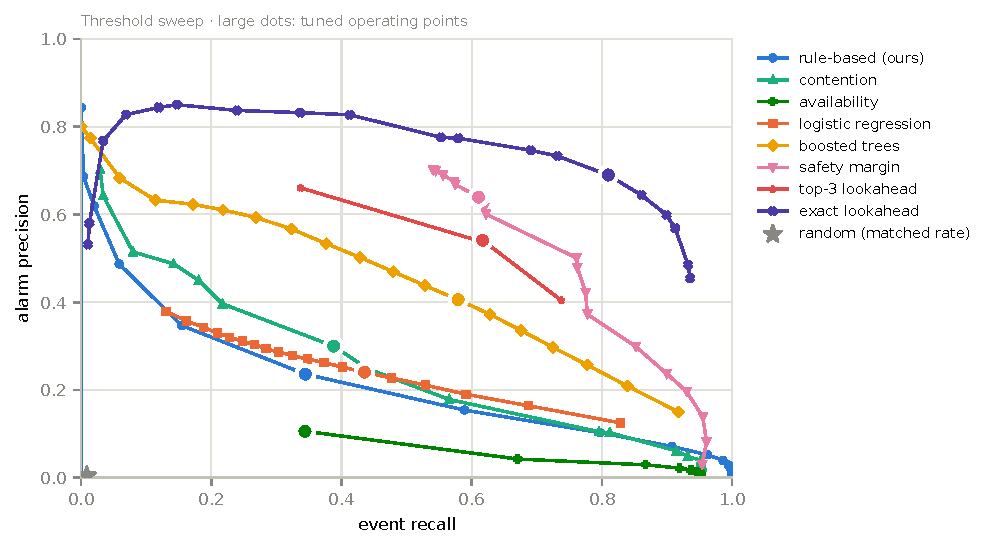
\includegraphics[width=\columnwidth]{fig3_pr_curves.pdf}
\caption{Precision--recall along each threshold sweep (test split).}\label{fig:pr}
\end{figure}

\finding{1}{In these configurations the rule-based score warned a median 10 steps ahead with F1 0.28, ahead of the free-resource threshold (0.16) and matched-rate random alarms (0.006) in 20 of 20 seed batches. Contention alone (0.34) and boosted trees on the same signals (0.48) did better.}

\subsection{Where Warning Quality Varies}\label{sec:res-workload}
Warning quality depended on how danger built up (Table~\ref{tab:scenario}). The rule-based score reached F1 0.42 on spike workloads but 0.22 and 0.23 on the gradual normal and deadlock-prone workloads. In spike sequences, unsafe onsets followed a median 26 steps after the spike began and 3.0\% occurred before it, so the abrupt change in request pattern gives the cheap signals time to react. The state-based checks kept a large advantage on the gradual workloads (safety margin 0.55 and 0.54). F1 of most methods was lower at $n=200$ than at small sizes (anomaly A4, Section~\ref{sec:anomalies}), and waiting ratio reversed its usual standing on spike workloads (anomaly A1).

\begin{table}[t]
\centering
\footnotesize
\caption{F1 PER WORKLOAD (UNSAFE TRANSITIONS, 20-STEP HORIZON).}
\label{tab:scenario}
\begin{tabular}{lrrr}
\toprule
Method & Normal & Bursty & Deadlock-prone \\
\midrule
Rule-based (ours) & 0.22 & 0.42 & 0.23 \\
Rule-based, max & 0.21 & 0.49 & 0.22 \\
Demand ratio & 0.06 & 0.34 & 0.01 \\
Contention & 0.21 & 0.49 & 0.22 \\
Blocked-process ratio & 0.29 & 0.03 & 0.31 \\
Request rate & 0.00 & 0.23 & 0.00 \\
Free-resource threshold & 0.10 & 0.34 & 0.05 \\
Logistic regression & 0.22 & 0.44 & 0.23 \\
Boosted trees & 0.36 & 0.58 & 0.43 \\
Safety margin & 0.55 & 0.78 & 0.54 \\
Partial lookahead & 0.45 & 0.80 & 0.44 \\
Full lookahead$^\dagger$ & 0.66 & 0.83 & 0.69 \\
Random & 0.00 & 0.01 & 0.01 \\
\bottomrule
\end{tabular}
\\[2pt]{\scriptsize $^\dagger$ common subset only.}
\end{table}


\finding{2}{Warning quality depended on the workload: the rule-based score reached F1 0.42 on spike workloads and 0.22--0.23 on gradual ones, where state-based checks kept a large advantage.}

\subsection{Cost--Accuracy Frontier}\label{sec:res-frontier}
Table~\ref{tab:cost} and Fig.~\ref{fig:frontier} relate accuracy to compute. One safety check took 59.9\,$\mu$s on average and one simulation step 289.2\,$\mu$s. The safety margin's seven checks cost 1.66 simulation steps at $n=200$ and the top-3 lookahead 0.91; their number of checks does not grow with $n$. Exact lookahead, one check per running process, cost 43.45 at $n=200$. These costs are a property of our instrument---a NumPy-vectorised check in Python---not of the algorithms: an incremental safety test~\cite{Belik1987,Finkel1987} or a compiled implementation would move every state-based point, so the ratios, not the absolute times, are the result, and even the ratios are untested on a second implementation.

On the common subset, the safety margin was lower than exact lookahead by 0.027 [0.023, 0.031] in all 20 batches; the difference is not zero. Its 90\% interval, $[-0.030, -0.024]$, lies inside $\pm0.05$, so the two are equivalent at that margin ($p_{\mathrm{TOST}}<0.001$); they would be equivalent at any $\delta$ above 0.030, and not below. The top-3 lookahead was lower by 0.052 and is not equivalent at $\delta=0.05$ ($p_{\mathrm{TOST}}=0.87$). Since $\delta$ was fixed after the point estimates were known, H2 is supported only as an exploratory result.

The state-based checks bought their accuracy with later warnings (Fig.~\ref{fig:leadprec}). Their median lead was 4--5 steps against 7--13 for the cheap signals. On the 17,648 onsets that both captured, the rule-based score warned a median 9 steps ahead and the safety margin 3; on the 8,012 onsets captured by both it and exact lookahead, 5 and 4 steps.

\begin{table}[t]
\centering
\footnotesize
\caption{MEASURED COMPUTE PER STEP, IN MICROSECONDS AND AS A MULTIPLE OF ONE SIMULATION STEP (WHICH INCLUDES ONE SAFETY CHECK AND THE INDICATORS).}
\label{tab:cost}
\begin{tabular}{lrrrr}
\toprule
 & \multicolumn{2}{c}{Average over sizes} & \multicolumn{2}{c}{$n=200$} \\
\cmidrule(lr){2-3}\cmidrule(lr){4-5}
Computation & $\mu$s & $\times$ step & $\mu$s & $\times$ step \\
\midrule
Simulation step & 289 & 1.00 & -- & -- \\
One safety check & 60 & 0.21 & -- & -- \\
Safety margin & 417 & 1.44 & 479 & 1.66 \\
Top-3 lookahead & 231 & 0.80 & 264 & 0.91 \\
Exact lookahead & 1{,}850 & 6.40 & 12{,}566 & 43.45 \\
\bottomrule
\end{tabular}
\end{table}

\begin{figure}[t]\centering
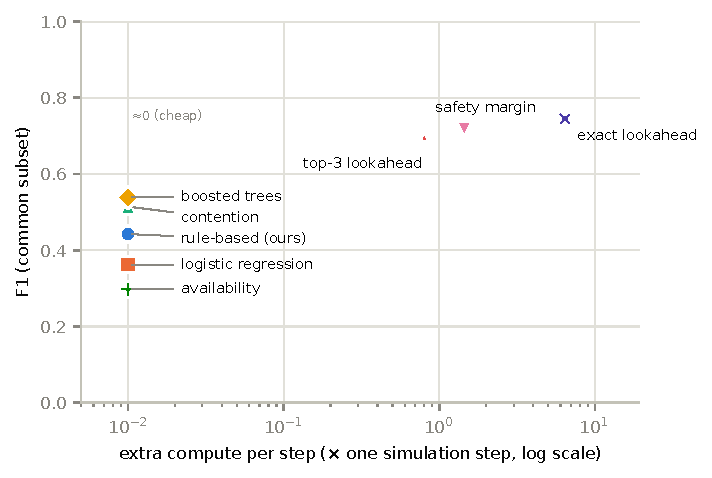
\includegraphics[width=\columnwidth]{fig9_cost_frontier.pdf}
\caption{F1 on the common subset against extra compute per step, averaged over system sizes (log scale).}\label{fig:frontier}
\end{figure}
\begin{figure}[t]\centering
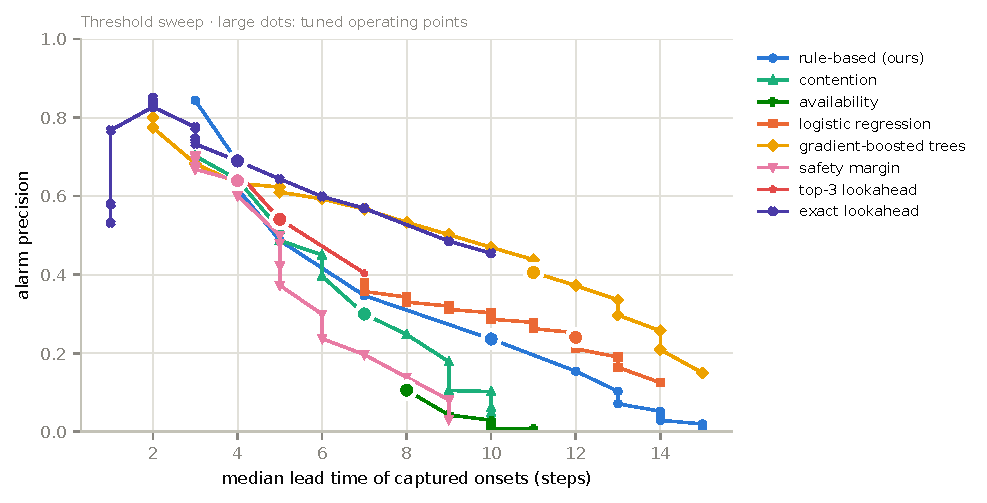
\includegraphics[width=\columnwidth]{fig10_precision_lead.pdf}
\caption{Precision against median lead time along each threshold sweep.}\label{fig:leadprec}
\end{figure}

\finding{3}{On the common subset the safety margin reached F1 0.72 and exact lookahead 0.74, at 1.7$\times$ and 43.5$\times$ one simulation step for 200 processes in our implementation. The margin was reliably lower by 0.027 but equivalent within a post-hoc $\pm0.05$. State-based checks warned later (median 4--5 steps) than the cheap signals (7--13).}

\subsection{Unsafe States and Deadlock}\label{sec:res-deadlock}
In this simulator, all resolved unsafe episodes ended in deadlock under the spike (29,868) and deadlock-prone (31,219) workloads, and 77\% under normal (16,613 of 21,525; Table~\ref{tab:episodes}). This follows partly from the design---processes eventually request their full claims, and a sequence ends at its first deadlock---and is a property of the model, not evidence about real systems (Section~\ref{sec:threats}).

For the deadlock-onset target, a comparison across the full population would mix populations, because exact lookahead covers 25,862 onsets and the other methods 77,700. Table~\ref{tab:deadlock} therefore reports every method on the common subset, with full-population F1 alongside. On identical sequences the rule-based score led with F1 0.659, followed by availability (0.552) and boosted trees (0.540); in the full population, waiting ratio and boosted trees had led (0.476). The three state-based checks (exact lookahead 0.369, safety margin 0.342, top-3 0.301) were behind every other method except request rate and random, the reverse of their standing on the unsafe target (anomaly A3).

\begin{table}[t]
\centering\footnotesize
\caption{PREDICTING DEADLOCK ONSETS UP TO 20 STEPS AHEAD. PRECISION, RECALL AND F1 ON THE COMMON SUBSET (25,862 ONSETS, ALL METHODS ON THE SAME SEQUENCES); LAST COLUMN: F1 ON THE FULL POPULATION (77,700 ONSETS).}
\label{tab:deadlock}
\begin{tabular}{lcccc}
\toprule
 & \multicolumn{3}{c}{Common subset} & Full \\
\cmidrule(lr){2-4}
Method & Precision & Recall & F1 & F1 \\
\midrule
Rule-based (ours) & 0.582 & 0.759 & 0.659 & 0.326 \\
Availability & 0.523 & 0.585 & 0.552 & 0.161 \\
Boosted trees & 0.374 & 0.969 & 0.540 & 0.476 \\
Contention & 0.390 & 0.772 & 0.518 & 0.262 \\
Need pressure & 0.621 & 0.426 & 0.505 & 0.235 \\
Waiting ratio & 0.413 & 0.499 & 0.452 & 0.476 \\
Logistic regression & 0.242 & 0.920 & 0.384 & 0.286 \\
Exact lookahead & 0.320 & 0.434 & 0.369 & -- \\
Safety margin & 0.317 & 0.370 & 0.342 & 0.155 \\
Top-3 lookahead & 0.269 & 0.343 & 0.301 & 0.128 \\
Request rate & 0.242 & 0.174 & 0.202 & 0.064 \\
Random & 0.030 & 0.009 & 0.014 & 0.006 \\
\bottomrule
\end{tabular}
\end{table}
\begin{table}[t]
\centering
\footnotesize
\caption{HOW UNSAFE EPISODES ENDED, PER WORKLOAD. AN EPISODE ``RECOVERS'' IF THE STATE BECOMES SAFE AGAIN.}
\label{tab:episodes}
\begin{tabular}{lrrr}
\toprule
Workload & Recovered & Deadlocked & \% deadlocked \\
\midrule
Normal & 4{,}912 & 16{,}613 & 77 \\
Bursty & 0 & 29{,}868 & 100 \\
Deadlock-prone & 0 & 31{,}219 & 100 \\
\bottomrule
\end{tabular}
\end{table}


\finding{4}{Under this simulator, 77--100\% of unsafe episodes ended in deadlock, partly by design. On identical sequences the rule-based score anticipated deadlock onsets best (F1 0.66) and the state-based checks were among the weakest (0.30--0.37).}

\subsection{Robustness to Misdeclared Claims}\label{sec:res-robust}
With every claim entry independently multiplied by a factor drawn from $[0.8, 1.2]$ for the indicators, while ground truth used the true claims, F1 changed by at most 0.004 for every claim-based method (Table~\ref{tab:robust}), which supports H3 as stated. The test is weak, however: the errors are independent and zero-mean, so they largely cancel in sums over processes and resource types. It says nothing about systematic misdeclaration, for example every process under-claiming by 20\%, which was not tested.

\begin{table}[t]
\centering
\footnotesize
\caption{ROBUSTNESS: F1 OF THE SAME TUNED METHODS WHEN EACH DECLARED CLAIM ENTRY IS RANDOMLY OFF BY UP TO $\pm$20\% (GROUND TRUTH USES THE TRUE CLAIMS).}
\label{tab:robust}
\begin{tabular}{lrrr}
\toprule
Method & True claims & Claims $\pm$20\% & Change \\
\midrule
Rule-based (ours) & 0.280 & 0.280 & +0.000 \\
Rule-based, max & 0.338 & 0.337 & $-$0.001 \\
Demand ratio & 0.190 & 0.194 & +0.004 \\
Contention & 0.338 & 0.337 & $-$0.001 \\
Logistic regression & 0.310 & 0.311 & +0.002 \\
Boosted trees & 0.477 & 0.476 & $-$0.001 \\
\bottomrule
\end{tabular}
\end{table}


\finding{5}{Unbiased per-entry claim error of up to $\pm$20\% changed F1 by at most 0.004; biased misdeclaration was not tested.}

\subsection{Horizon Sensitivity}\label{sec:res-horizon}
Scoring the same alarms against wider horizons raised every method's F1 (Table~\ref{tab:hmax}); the rule-based score rose from 0.108 at $H_{\max}=5$ to 0.399 at 50: many alarms counted as false at the 20-step horizon in fact precede an onset by 21 to 50 steps. The ranking of the methods in Table~\ref{tab:hmax} did not change.

\begin{table}[t]
\centering\footnotesize
\caption{F1 WHEN AN ALARM COUNTS AS CORRECT IF AN UNSAFE ONSET FOLLOWS WITHIN 5, 10, 20 OR 50 STEPS (SAME ALARMS).}
\label{tab:hmax}
\begin{tabular}{lcccc}
\toprule
Method & 5 steps & 10 & 20 & 50 \\
\midrule
Rule-based (ours) & 0.108 & 0.190 & 0.280 & 0.399 \\
Contention & 0.129 & 0.222 & 0.338 & 0.432 \\
Boosted trees & 0.178 & 0.330 & 0.477 & 0.597 \\
Safety margin & 0.374 & 0.490 & 0.625 & 0.707 \\
Top-3 lookahead & 0.295 & 0.433 & 0.576 & 0.691 \\
Exact lookahead$^\dagger$ & 0.482 & 0.648 & 0.745 & 0.798 \\
Availability & 0.055 & 0.097 & 0.162 & 0.251 \\
Random & 0.002 & 0.003 & 0.006 & 0.015 \\
\bottomrule
\end{tabular}
\\[2pt]{\scriptsize $^\dagger$ common subset only.}
\end{table}

\finding{6}{Widening the horizon from 5 to 50 steps raised every method's F1 (rule-based 0.11 to 0.40) without changing their ranking.}

\subsection{Scaling of the Safety Check}\label{sec:res-scaling}
On random valid states, the vectorised safety check was 1.4--7.7 times faster than the textbook loop (Table~\ref{tab:scaling}, Fig.~\ref{fig:scaling}). Its time grew with a log--log slope of 0.27 in $n$ at $m=20$, against 0.76 for the reference loop, far below the $\Theta(mn^2)$ worst case. This is the average-case behaviour of one implementation on these states.

\begin{table}[!htb]
\centering
\scriptsize
\caption{TIME PER BANKER'S SAFETY CHECK ON RANDOM VALID STATES: OUR VECTORISED NUMPY VERSION AGAINST THE TEXTBOOK LOOP.}
\label{tab:scaling}
\begin{tabular}{rrrrr}
\toprule
$n$ & $m$ & Vectorised ($\mu$s) & Textbook ($\mu$s) & Speed-up \\
\midrule
10 & 5 & 7.1 & 9.7 & 1.4 \\
10 & 10 & 6.9 & 9.4 & 1.4 \\
10 & 20 & 6.9 & 10.5 & 1.5 \\
25 & 5 & 9.0 & 19.5 & 2.2 \\
25 & 10 & 7.4 & 17.6 & 2.4 \\
25 & 20 & 7.4 & 17.3 & 2.3 \\
50 & 5 & 9.1 & 29.6 & 3.3 \\
50 & 10 & 8.1 & 28.4 & 3.5 \\
50 & 20 & 9.0 & 28.6 & 3.2 \\
100 & 5 & 12.1 & 60.8 & 5.0 \\
100 & 10 & 9.9 & 51.9 & 5.3 \\
100 & 20 & 11.2 & 54.3 & 4.9 \\
200 & 5 & 17.8 & 138.0 & 7.7 \\
200 & 10 & 13.7 & 103.3 & 7.6 \\
200 & 20 & 15.6 & 99.7 & 6.4 \\
\bottomrule
\end{tabular}
\end{table}

\begin{figure}[t]\centering
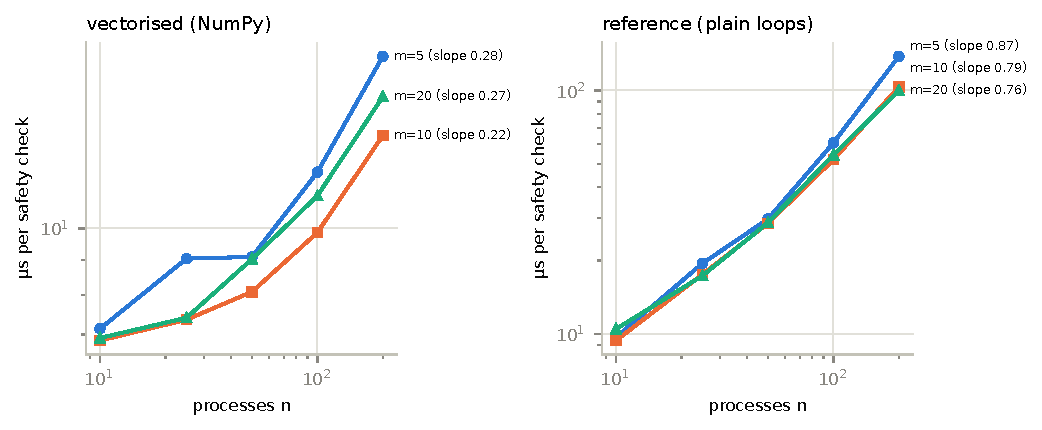
\includegraphics[width=\columnwidth]{fig7_scaling.pdf}
\caption{Time per safety check against $n$ (log--log).}\label{fig:scaling}
\end{figure}

\finding{7}{The vectorised safety check grew far more slowly than $\Theta(mn^2)$ in these workloads (slope 0.27 at $m=20$); this is average-case behaviour of one implementation.}

\subsection{Open Anomalies}\label{sec:anomalies}
Six observations are not explained by anything above.

\textbf{(A1)} Waiting ratio reached F1 0.29 on normal and 0.31 on deadlock-prone workloads but 0.03 on spike workloads, where it raised 1,402 alarms for 29,868 onsets. A plausible cause is that spike grabs are capped by free units and therefore granted, so few processes block before the onset; we have not traced waiting counts before onsets to check this.

\textbf{(A2)} Boosted trees reached recall 0.985 on the deadlock target in the full population (0.992 at $H_{\max}=50$) and 0.969 on the common subset, with precision 0.31--0.37; no other method approached this recall. Because alarms are not suppressed during unsafe episodes for this target, the model may simply alarm throughout the unsafe stretch that precedes deadlock. Restricting the analysis to alarms raised while safe would test this.

\textbf{(A3)} The state-based checks led on the unsafe target but were among the weakest methods on the deadlock target, on identical sequences (Table~\ref{tab:deadlock}). All three are computed only on safe steps, so they are silent during the unsafe episodes that precede deadlock; this is likely a construction effect rather than a property of the signals, and computing them on unsafe steps too would resolve it.

\textbf{(A4)} F1 of the state-based checks and boosted trees fell steadily with size (exact lookahead 0.756 at $n=10$ to 0.534 at $n=200$, safety margin 0.722 to 0.509, boosted trees 0.568 to 0.410), and the rule-based score fell from 0.470 at $n=25$ to 0.197 (0.433 at $n=10$). Waiting ratio moved the other way, from 0.087 at $n=10$ to 0.312 at $n=100$ (0.270 at 200), and need pressure and availability peaked at $n=50$. Thresholds were tuned once across sizes and onset density differs by size; per-size tuning would separate the two.

\textbf{(A5)} Request rate scored F1 0.001 on normal and 0.000 on deadlock-prone workloads against 0.23 on spike, and need pressure 0.01 on deadlock-prone; three single-indicator baselines chose the top of the threshold grid (95), so their best operating point may lie outside the grid.

\textbf{(A6)} Logistic regression raised 5.44 false alarms per 1,000 steps on the common subset against 0.48 on the full population, above the tuning constraint of five. Thresholds tuned on all sizes may not transfer to the small systems that dominate the subset; per-size tuning (A4) would test this too.

% =============================================================================
\section{Threats to Validity}\label{sec:threats}
\textbf{Internal.} The seed batches replicate test-side sampling from one generator with thresholds tuned once; they do not capture variation from re-tuning or from a different generator. The hypotheses, the equivalence margin and several analyses were chosen after the data were seen. Two pipeline bugs were fixed mid-run, the spike workload was redesigned after calibration and the tuning split was reduced (Section~\ref{sec:stats}).

\textbf{External.} The workloads are synthetic, claims are declared and the process set is fixed. One simulator and one NumPy implementation were used, so the cost results are an instrument effect (Section~\ref{sec:res-frontier}), on one instance type in one region. The 77--100\% unsafe-to-deadlock rate follows partly from the design, since processes eventually request their full claims and sequences end at the first deadlock; in systems where processes stop short of their claims, fewer unsafe states would become deadlocks.

\textbf{Construct.} F1 at a 20-step horizon is one operating point. ``Moderate'' precision is judged against clinical early warning~\cite{Hyland2020}. The safety margin is a scalar, proportional form of Finkel and Madduri's measure, not their algorithm. ``Unsafe'' is Banker's pessimistic notion, not imminent deadlock.

\textbf{Experiments not run.} The claims of this paper are limited by the following:
\begin{enumerate}
\item real allocation traces: public cluster traces do not record per-process maximum claims or hold-and-wait sequences, so Banker ground truth cannot be derived from them;
\item biased claim misdeclaration (all claims scaled by a common factor);
\item re-tuning per batch, which would make each batch a full replication;
\item two-stage gating, in which the cheap score triggers the safety margin;
\item a second implementation of the safety check, such as an incremental test, to separate algorithm from instrument;
\item a pre-registered confirmatory campaign with the hypotheses, $\delta$ and batch count fixed in advance;
\item the checks proposed for anomalies A1--A6.
\end{enumerate}

% =============================================================================
\section{Discussion and Conclusion}\label{sec:conclusion}
Three things came out of the measurements that the simple estimate of Section~\ref{sec:intro} could not have told us. First, warning quality depended on the regime: cheap signals did well when danger built up abruptly and poorly when it built up gradually, and most methods degraded in larger systems, while waiting ratio improved. Second, two of our initial expectations were partly wrong: averaging indicators did worse than the strongest indicator alone, and the pilot run had suggested that exact lookahead warns much later than the cheap score (median 3 versus 7 steps), whereas in the main run the paired leads were 4 and 5. Third, the cheap signals hold more than a weighted sum extracts---boosted trees on the same features reached 0.48 against 0.28---and the ranking of methods depends on the population and the target: on identical sequences, the rule-based score anticipated deadlock onsets better than any state-based check.

For a practitioner, the measurements suggest a procedure: run a cheap score continuously and, when it crosses its threshold, evaluate the safety margin, which costs a fixed seven safety checks per step and in these configurations comes within 0.03 F1 of exact lookahead; for small systems, exact lookahead itself is affordable. The cheap score supplies the earlier warning and the state check the precision. This procedure follows from the components' measurements; it was not tested end to end.

For designers of warning methods, the lesson is to compare methods on identical populations, with paired replicates, and to report compute cost and lead time alongside accuracy. In this study each of these changed a conclusion: population mixing hid the deadlock-target ranking, cost separated two methods within 0.03 F1 of each other, and lead time reversed the order of the cheap and state-based methods.

These results come from one simulator, synthetic workloads with declared claims, one implementation and one cloud instance. They do not establish behaviour on real allocators, under biased claims or in distributed settings.

\section*{Data and Code Availability}
The simulator, configurations, analysis scripts (including \texttt{analysis/batches.py} for the batch, equivalence and common-subset analyses), per-sequence evaluation rows and a sample of per-step traces are in the authors' repository and are available from the authors on request. Configurations record seeds, configuration hashes and commit identifiers (exploratory run \texttt{d3de8e5}; main run \texttt{328caf6} with the fix of \texttt{173a323}).

\bibliographystyle{IEEEtran}
\bibliography{../refs}

\end{document}
